\section{QUIC and ECH}

In combination with HTTP, the TLS protocol provides security by encrypting the HTTP payload.
Unlike HTTP versions 1 and 2, which operate over TCP (and may or may not use a TLS layer),
HTTP version 3, standardised in 2022, is designed to use QUIC as a transport.
Rather than forming a separate layer, TLS is tightly integrated with QUIC, and QUIC and TLS components are expected to cooperate, as illustrated in Figure~\ref{fig:quic-tls}.

QUIC can provide a reliable stream abstraction to applications in a similar way to TCP, and this is how it is expected to operate with TLS.
RFC 9001~\cite{rfc9001} describes in detail how TLS is used to secure the QUIC transport protocol.

\begin{figure}[h]
    \centering
    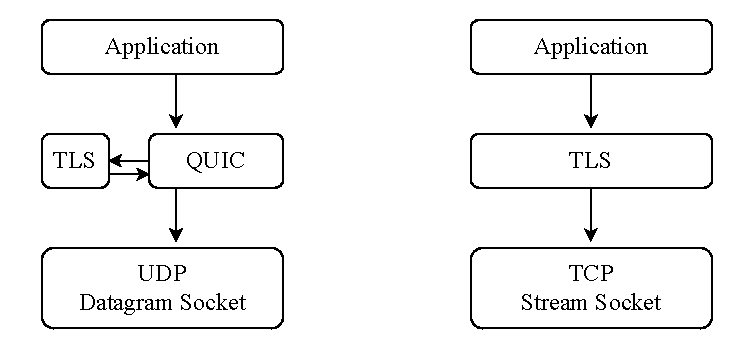
\includegraphics[width=0.75\linewidth]{quic_and_ech/figs/QUIC-TLS.pdf}
    \caption{Compared to the strict layering of TLS and TCP, QUIC and TLS components are expected to cooperate.}
    \label{fig:quic-tls}
\end{figure}

Implementing ECH in the various QUIC software is expected to rely on enabling it in the underlying SSL library, similar to providing it for TCP, and then calling the relevant functions from the library on connection setup.
Some differences exist, as QUIC also needs to configure TLS.

The interface between QUIC and TLS includes sending and receiving handshake messages~\cite{rfc9001}:
a QUIC client requests TLS handshake bytes from the TLS implementation, while a QUIC server provides the TLS layer with the client's handshake bytes. QUIC carries this TLS handshake data in CRYPTO frames, directly over the QUIC transport, which substitutes the TLS record layer (required when transmitting data over TCP, as TCP does not have framing capabilities).
In exchange, TLS provides QUIC with cryptographic keys and state change information.

QUIC can use 2 handshake modes:
\begin{itemize}
    \item  A 1 Round Trip Time (1-RTT) handshake, where application data is sent after the server has responded to the first handshake message from the client
     \item A 0-RTT handshake where application data is immediately sent, e.g. right after the client sends/server receives a TLS ClientHello
\end{itemize}

Once the TLS handshake is complete, QUIC can send application data. This is carried in Stream frames rather than in TLS Application Data records. TLS then does not send more data unless requested (e.g., as noted in~\cite{rfc9001}, if the server wishes to provide additional or updated session tickets to a client).
